\chapter*[Conclusão]{Conclusão}\addcontentsline{toc}{chapter}{Conclusão}\label{conclusao}

Estimulada por artistas-programadores(as), a interiorização de um processo criativo (bricolagem) pode ter conduzido à formação de programas de pesquisas interdisciplinares no Norte global. Isto é, teorias das Artes Músicais, Audiovisuais, Corporais, Têxteis, Filosofia, e se a criatividade permitir, da Engenharia Crítica, são coisificadas para elaboração de novos conceitos. Uma classe particular de artistas-programadores(as) \cite[p.~16]{McLean2011}, o(a) improvisador(a) de códigos (\emph{live coder}), admite conhecimentos da engenharia de computação, revisada sob o prisma de uma ou mais teorias   como extensão para improvisações ou ou análise de registros.

O \emph{live coder} é aquele que pratica o \emph{live coding} como divulgado em uma página da Internet\disponivelem{http://www.toplap.org} e uma publicação \cite{ward_live_2004}; também se mantêm informado das publicações que investigam o \emph{live coding}, como em revistas acadêmicas como \emph{Computer Music Journal}, \emph{Leonardo}, listas de email de \emph{softwares}, páginas do Google, e improvisa programas com fins pedagógicos, musicais, audiovisuais, têxteis e filosóficos. O improvisador de códigos pratica o \emph{live coding}:

%Por exemplo, um duo de improvisadores-programadores (\emph{live coders}), cada um com sua programação-partitura\footnote{\cfcite[p.~5]{fenerich_marulho_2014}.}, executam uma performance artítica \ver{fig:toalete}.

%\begin{figure}[h]
%    \centering
%    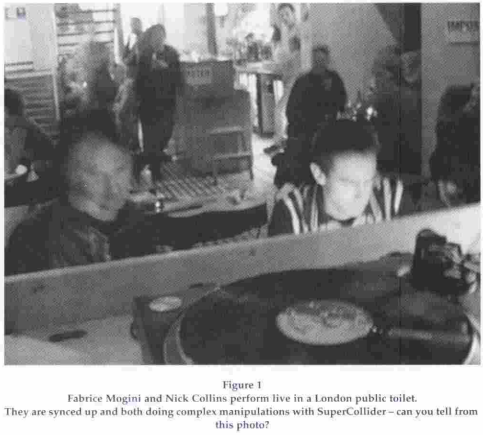
\includegraphics[scale=0.71]{imagens/toalete.png}
%    \caption{ ``Fabrice Mogini e Nick Collins tocando ao vivo em um banheiro público de Londres. Eles estão sincronizados e ambos fazendo manipulações complexas com o \emph{SuperCollider}.''. \textbf{Fonte}: \citeonline{collins_generative_2003}.}
%    \label{fig:toalete}
%  \end{figure}


\begin{citacao}
\emph{Programação imediata} (ou: programação de conversa, programação no fluxo, programação interativa) é um paradigma que inclue a atividade de programação ela mesma como uma operação do programa. Isto significa um programa que não é tomado como ferramenta que cria primeiro, e depois é produtivo, mas um processo de construção dinâmica de descrição e conversação - escrever o código e então se tornar parte da prática musical ou experimental. \cite[Verbete JITLib]{supercollider.org_supercollider_2014}\footnote{Tradução de \emph{Just in time programming (or: conversational programming, live coding , on-the fly-programming, interactive programming) is a paradigm that includes the programming activity itself in the program's operation. This means a program is not taken as a tool that is made first, then to be productive, but a dynamic construction process of description and conversation - writing code thus becoming a closer part of musical or experimental practice.}}
\end{citacao}

\citeonline{ward_live_2004} definem a improvisação de códigos como \traducao{atividade da escrita integral (ou partes) de um programa enquanto ele é executado}{Live coding is the activity of writing (parts of ) a program while it runs}. \citeonline{blackwell_programming_2005} enfatizam a definição do ponto de vista da linguagem de programação como instrumento musical. \citeonline{mclean_hacking_2006} relata o \emph{live coding} como ferramenta para um \emph{Disk Jockey codificado}.  \citeonline{sorensen_keith_2009} pontuam a improvisação de códigos como \traducao{uma prática de performance para o qual linguagens de computador definem o meio primário de expressão artística.}{Live coding is a performance pratice for which computer languages define  the primary means of expression.}. Para \citeonline{sorensen_impromptu_2010}, \emph{live coding} (ou \emph{livecoding}) envolve a premissa de uma programação-partitura audiovisual reativa: 

\traduzcitacao{
Livecoding é uma prática de arte computacional que envolve criação em tempo-real de programas de audiovisual generativo para performances multimídias interativas. Comumente as ações dos programadores são expostas para uma audiência por projeção do ambiente de edição. Performances de livecoding geralmente envolvem mais de um participante, e são geralmente iniciadas a partir de uma folha conceitual em branco   
}{Livecoding [10, 50] is a computational arts practice that involves the real-time creation of generative audiovisual software for interactive multimedia performance. Commonly the programmers’ actions are exposed to the audience by projection of the editing environment. Livecoding performances often involve more than one participant, and are often commenced from a conceptual blank slate}
{p.~823}
{sorensen_impromptu_2010}

\citeonline{magnusson_algorithms_2011,collins_origins_2014} sintetizam o \emph{live coding} como improvisação audiovisual. \citeonline{sorensen_programming_2014} define como \traducao{programar sistemas de tempo-real em tempo real}{programming real-time systems in real-time}. Em um discussão entitulada ``\emph{Wtf is livecoding}''\disponivelem{http://lurk.org/groups/livecode/messages/topic/ofAxZpxsKFpDRLnoA48Bh} diz que o \traducao{\emph{Live coding} celebra a efemeridade da própria definição}{Live coding celebrates the ephemerality of definition itself} \ver{fig:live_coding_def}.

Embora semelhantes, as definições mudam de detalhes de acordo com o contexto. Por exemplo, \citeonline{ward_live_2004} enfatizam que o código pode ser (re)composto de partes menores. \citeonline{mclean_hacking_2006} enfatiza algum onde um código é (re)programado. \citeonline{sorensen_programming_2014} enfatiza que modificar algo é próprio da técnica, em seus significados técnicos. O compositor Nick Collins situa que a definição nunca deve ser uma constante, e sim caracterizada em função do contexto. 

  \begin{figure}[h]
    \centering
    
\includegraphics[scale=0.7]{imagens/live_coding_def.png}
    \caption{Definição de \emph{live coding}: ``Insira a definição aqui''. \textbf{Fonte}: \citeonline{collins_origins_2014}.}
    \label{fig:live_coding_def}
  \end{figure}


Se por um lado a definição agrega definições, o que dificulta a tarefa inicial de descrever os fundamentos objeto de pesquisa, por outro ilustra a improvisação de códigos como um \emph{Universo de conceitos}. Neste trabalho consideramos que definições ou performances de improvisação de códigos estão contidas em diferentes \emph{Espaços Conceituais} \cite{wiggins_framework_2006,mclean_music_2006}. Artistas-programadores (\emph{live coders}) transitam entre os Espaços Conceituais para criação de Sistemas Criativos (códigos, programas). Estes Sistemas Criativos são representados em diferentes Linguagens de Programação. Regras práticas conduzem o processo de escrita e exposição desta linguagem; mas n1ão restringem o resultado (no caso da pesquisa, musical). Mas algumas categorizações musicais se destacam.  Neste sentido, selecionamos um exemplo simbólico, \emph{A Study in Keith} de Andrew \citeonline{sorensen_keith_2009}\footnote{Disponível em \url{https://vimeo.com/2433947}.}. Representa um caso particular que foge dos exemplos citados anteriormente, mas envolve a manutenção de uma tradição musical tonal através de um interessante esforço de \emph{replicação do estilo}. 

No \autoref{cap:introducao} selecionamos algumas abordagens de uma grande quantidade de exemplos possíveis. Foram escolhidos por manterem alguma conexão com a improvisação de códigos no contexto sonoro. De certa forma, induzimos conceitos ligados à Música.  No \autoref{cap:metodologia} apresentamos um modelo de formalização dEspaços conceituais observados pelo prisma do Modelo de Improvisação discutido por Alex \citeonline{mclean_music_2006}. No \autoref{cap:estudos_de_caso}, organizamos conceitos de uma sonoridade-algoritmo inicial de \emph{A Study in Keith} segundo este modelo. Por último uma conclusão, mais uma reflexão sobre o processo de pesquisa do que obtenção de um resultado final. Dois apêndices foram adicionados para exposição do material que estimulou o interesse pelo tema discutido.